% !TeX root = construct.tex


\selectlanguage{hebrew}
\chapter{אמא'לה, המחוגה שלי התמוטטה!}\label{c.collapse}

%%%%%%%%%%%%%%%%%%%%%%%%%%%%%%%%%%%%%%%%%%%%%%%%%%%%%%%%%%%%%%%

\section{
\R{מחוגה קבועה ומחוגה מתמוטטת}
}

במחוגה מודרנית ניתן לקבע את המרחק בין שתי הרגליים, וכך להעתיק קטע קו או מעגל ממקום למקום. נקרא למחוגה זו: "מחוגה קבועה". בספרי לימוד גיאומטריה ניתן למצוא בנייה של אנך אמצעי לקטע קו על ידי בניית שני מעגלים שמרכזם על הקו, ובלבד שהרדיוס
\textbf{גדול ממחצית המרחק בין המרכזים},
כפי שניתן לראות בתרשים השמאלי:
\begin{center}
\selectlanguage{english}
\begin{tikzpicture}[scale=0.5]
\begin{scope}
\coordinate (A) at (0,0);
\coordinate (B) at (4,0);
\draw ($(A)!-.3!(B)$) -- ($(A)!1.3!(B)$);
\fill (A) node[below] {$A$}circle[radius=3pt];
\fill (B)  node[below] {$B$} circle[radius=3pt];
\draw[name path=larc] (A) ++(-60:3cm) arc (-60:60:3cm);
\draw[name path=rarc] (B) ++(-120:3cm) arc (-120:-240:3cm);
\path [name intersections={of=larc and rarc,by={b,t}}];
\fill (t) node[above right,xshift=-2pt,yshift=5pt] {$C$} circle[radius=3pt];
\fill (b) node[below left,xshift=2pt,yshift=-5pt] {$D$} circle[radius=3pt];
\draw ($ (b) ! 1.2 ! (t)$) -- ($ (t) ! 1.2 ! (b)$);
\end{scope}
\begin{scope}[xshift=12cm]
\coordinate (A) at (0,0);
\coordinate (B) at (4,0);
\draw ($(A)!-.3!(B)$) -- ($(A)!1.3!(B)$);
\fill (A) node[below left] {$A$}circle[radius=3pt];
\fill (B)  node[below right] {$B$} circle[radius=3pt];
\draw[name path=larc] (A) ++(-80:4cm) arc (-80:80:4cm);
\draw[name path=rarc] (B) ++(-100:4cm) arc (-100:-260:4cm);
\path [name intersections={of=larc and rarc,by={b,t}}];
\fill (t) node[above right,xshift=-2pt,yshift=3pt] {$C$} circle[radius=3pt];
\fill (b) node[below left,xshift=2pt,yshift=-3pt] {$D$}circle[radius=3pt];
\draw ($ (b) ! 1.2 ! (t)$) -- ($ (t) ! 1.2 ! (b)$);
\end{scope}
\end{tikzpicture}
\end{center}

אוקלידס השתמש במחוגה "מתמוטטת" )%
\L{collapsing}%
(,
שרגליה מתקפלות כאשר מרימים אותה מהנייר. מחוגה המורכבת מגיר הקשור לחוט היא מחוגה מתמוטטת, כי אי-אפשר לשמור את הרדיוס כאשר מרימים אותה מהלוח. התרשים הימני למעלה מראה בנייה של אנך אמצעי באמצעות מחוגה מתמוטטת: האורך של
$AB$
שווה כמובן לאורך של
$BA$,
ולכן למעגלים רדיוס זהה.

הוכחת הנכונות של הבנייה הראשונה היא לא פשוטה, כי צריך להשתמש במושגים יחסית מתקדמים כגון משולשים חופפים. בבנייה השנייה קל להוכיח שמתקבל משולש שווה צלעות. האורך של
$AC$
שווה לאורכו של
$AB$,
כי שניהם רדיוסים של אותו מעגל, ומאותה סיבה האורך של
$BC$
שווה לאורכו של
$BA$.
מכאן:
\[
AC = AB = BA = BC\,.
\]

\vspace{-2ex}

\begin{center}
\selectlanguage{english}
\begin{tikzpicture}[scale=0.5]
\begin{scope}
\coordinate (A) at (0,0);
\coordinate (B) at (4,0);
\draw ($(A)!-.3!(B)$) -- ($(A)!1.3!(B)$);
\fill (A) node[below left] {$A$}circle[radius=3pt];
\fill (B)  node[below right] {$B$} circle[radius=3pt];
\draw[name path=larc] (A) ++(-60:3cm) arc (-60:60:3cm);
\draw[name path=rarc] (B) ++(-120:3cm) arc (-120:-240:3cm);
\path [name intersections={of=larc and rarc,by={b,t}}];
\fill (t) node[above right,xshift=-2pt,yshift=5pt] {$C$} circle[radius=3pt];
\fill (b) node[below left,xshift=2pt,yshift=-5pt] {$D$} circle[radius=3pt];
\draw (A) -- (t);
\draw (B) -- (t);
\end{scope}
\begin{scope}[xshift=12cm]
\coordinate (A) at (0,0);
\coordinate (B) at (4,0);
\draw ($(A)!-.3!(B)$) -- ($(A)!1.3!(B)$);
\fill (A) node[below left] {$A$}circle[radius=3pt];
\fill (B)  node[below right] {$B$} circle[radius=3pt];
\draw[name path=larc] (A) ++(-80:4cm) arc (-80:80:4cm);
\draw[name path=rarc] (B) ++(-100:4cm) arc (-100:-260:4cm);
\path [name intersections={of=larc and rarc,by={b,t}}];
\fill (t) node[above right,xshift=-2pt,yshift=3pt] {$C$} circle[radius=3pt];
\fill (b) node[below left,xshift=2pt,yshift=-3pt] {$D$}circle[radius=3pt];
\draw (A) -- (t);
\draw (B) -- (t);
\end{scope}
\end{tikzpicture}
\end{center}

\np

הבנייה של משולש שווה צלעות היא המשפט הראשון בספר של אוקלידס. המשפט השני מראה שאפשר להעתיק קטע קו עם מחוגה מתמוטטת, ולכן המחוגה הקבועה לא מוסיפה יכולת חדשה. 
\L{Toussaint} \L{\cite{toussaint}}
הראה שפורסמו הוכחות שגויות רבות של המשפט, ודווקא אוקלידס הוא זה שנתן הוכחה נכונה! אציג את הבנייה של אוקלידס ביחד עם הוכחת הנכונות. אחר כך אציג בנייה שגויה.
%%%%%%%%%%%%%%%%%%%%%%%%%%%%%%%%%%%%%%%%%%%%%%%%%%%%%%%%%%%%%%%

\section{%
העתקת קטע קו לפי אוקלידס%
}

\textbf{משפט:}
נתון קטע קו
$AB$
ונקודה
$C$
)תרשים משמאל(, ניתן לבנות )עם מחוגה מתמוטטת( בנקודה
$C$
קטע קו שאורכו שווה לאורכו של 
$AB$:


\begin{center}
\selectlanguage{english}
\begin{tikzpicture}[scale=0.4]
\begin{scope}
\coordinate (C) at (0,0);
\coordinate (A) at (2.5,0);
\coordinate (B) at (5.5,2);
\draw (A) node[below,xshift=-2pt,yshift=-2pt] {$A$} -- (B) node[right] {$B$};
\fill (A) circle[radius=3pt];
\fill (B) circle[radius=3pt];
\fill (C) node[below,xshift=2pt,yshift=-2pt] {$C$} circle[radius=3pt];
\end{scope}
\begin{scope}[xshift=12cm]
\coordinate (C) at (0,0);
\coordinate (A) at (2.5,0);
\coordinate (B) at (5.5,2);
\draw (A) node[below,xshift=-2pt,yshift=-2pt] {$A$} -- (B) node[right] {$B$};
\fill (A) circle[radius=3pt];
\fill (B) circle[radius=3pt];
\fill (C) node[below,xshift=2pt,yshift=-2pt] {$C$} circle[radius=3pt];
\draw (A) -- (C);
\path[name path=larc] (C) ++(-70:2.5cm) arc (-70:70:2.5cm);
\path[name path=rarc] (A) ++(-110:2.5cm) arc (-110:-250:2.5cm);
\path [name intersections={of=larc and rarc,by={d,D}}];
\fill (D) node[above] {$D$} circle[radius=3pt];
\draw (A) -- (D);
\draw (C) -- (D);
\end{scope}
\end{tikzpicture}
\end{center}

\vspace*{-6ex}
\textbf{%
הבנייה:%
}

חברו בקו את הנקודות
$A$
ו-%
$C$.

בנו משולש שווה צלעות שבסיסו
$AC$. 
לפי המשפט הראשון של אוקלידס הבנייה אפשרית עם מחוגה מתמוטטת. סמנו את הקודקוד של המשולש ב-%
$D$
)תרשים ימני למעלה(. 

בנו קרן בהמשך של
$DA$
וקרן בהמשך של 
$DC$
)התרשים משמאל(.


בנו מעגל שמרכזו 
$A$
עם רדיוס
$AB$.
סמנו
$E$,
החיתוך של המעגל עם הקרן
$DE$
)תרשים מימין(.


\begin{center}
\selectlanguage{english}
\begin{tikzpicture}[scale=0.4]
\begin{scope}
\coordinate (C) at (0,0);
\coordinate (A) at (2.5,0);
\coordinate (B) at (5.5,2);
\draw (A) node[below,xshift=-2pt,yshift=-2pt] {$A$} -- (B) node[right] {$B$};
\fill (A) circle[radius=3pt];
\fill (B) circle[radius=3pt];
\fill (C) node[below,xshift=2pt,yshift=-2pt] {$C$} circle[radius=3pt];
\draw (A) -- (C);
\path[name path=larc] (C) ++(-70:2.5cm) arc (-70:70:2.5cm);
\path[name path=rarc] (A) ++(-110:2.5cm) arc (-110:-250:2.5cm);
\path [name intersections={of=larc and rarc,by={d,D}}];
\fill (D) node[above] {$D$} circle[radius=3pt];
\draw (A) -- (D);
\draw (C) -- (D);
\draw[name path=ray2] (D) -- ($ (D) ! 3 ! (C) $);
\draw[name path=ray1] (D) -- ($ (D) ! 3 ! (A) $);
\end{scope}
\begin{scope}[xshift=12cm]
\coordinate (C) at (0,0);
\coordinate (A) at (2.5,0);
\coordinate (B) at (5.5,2);
\draw (A) node[below,xshift=-2pt,yshift=-2pt] {$A$} -- (B) node[right] {$B$};
\fill (A) circle[radius=3pt];
\fill (B) circle[radius=3pt];
\fill (C) node[below,xshift=2pt,yshift=-2pt] {$C$} circle[radius=3pt];
\draw (A) -- (C);
\path[name path=larc] (C) ++(-70:2.5cm) arc (-70:70:2.5cm);
\path[name path=rarc] (A) ++(-110:2.5cm) arc (-110:-250:2.5cm);
\path [name intersections={of=larc and rarc,by={d,D}}];
\fill (D) node[above] {$D$} circle[radius=3pt];
\draw (A) -- (D);
\draw (C) -- (D);
\draw[name path=ray2] (D) -- ($ (D) ! 3 ! (C) $);
\draw[name path=ray1] (D) -- ($ (D) ! 3 ! (A) $);
\node[draw,circle through=(B),name path=c1] at (A) {};
\path [name intersections={of=c1 and ray1,by={E,e}}];
\fill (E) node[right,xshift=2pt,yshift=-2pt] {$E$} circle[radius=3pt];
\end{scope}
\end{tikzpicture}
\end{center}

בנו מעגל שמרכזו 
$D$
עם רדיוס 
$DE$.
סמן את החיתוך של הקרן
$DC$
עם המעגל ב-%
$F$:


\begin{center}
\selectlanguage{english}
\begin{tikzpicture}[scale=0.4]
\coordinate (C) at (0,0);
\coordinate (A) at (2.5,0);
\coordinate (B) at (5.5,2);
\draw (A) node[below,xshift=-2pt,yshift=-2pt] {$A$} -- node[above] {$x$} (B) node[right] {$B$};
\fill (A) circle[radius=3pt];
\fill (B) circle[radius=3pt];
\fill (C) node[below,xshift=2pt,yshift=-2pt] {$C$} circle[radius=3pt];
\draw (A) -- (C);
\path[name path=larc] (C) ++(-70:2.5cm) arc (-70:70:2.5cm);
\path[name path=rarc] (A) ++(-110:2.5cm) arc (-110:-250:2.5cm);
\path [name intersections={of=larc and rarc,by={d,D}}];
\fill (D) node[above] {$D$} circle[radius=3pt];
\draw (A) -- node[right] {$y$} (D);
\draw (C) -- node[left] {$y$} (D);
\draw[name path=ray2] (D) -- ($ (D) ! 3 ! (C) $);
\draw[name path=ray1] (D) -- ($ (D) ! 3 ! (A) $);
\node[draw,circle through=(B),name path=c1] at (A) {};
\path [name intersections={of=c1 and ray1,by={E,e}}];
\fill (E) node[right,xshift=2pt,yshift=-2pt] {$E$} circle[radius=3pt];
\node[draw,circle through=(E),name path=c2] at (D) {};
\path [name intersections={of=c2 and ray2,by={F,f}}];
\fill (F) node[left,xshift=-2pt,yshift=-2pt] {$F$} circle[radius=3pt];
\path (A) -- node[right] {$x$} (E);
\path (C) -- node[left] {$x$} (F);
\end{tikzpicture}
\end{center}

\np

\textbf{טענה:}
אורכו של קטע הקו
$CF$
שווה לאורך קטע הקו
$AB$.


\textbf{הוכחה:}
$DC=DA$
כי
$\triangle ACD$
שווה צלעות.
$AE=AB$
כי שניהם רדיוסים של המעגל שמרכזו 
$A$.
$DF=DE$
כי שניהם רדיוסים של המעגל שמרכזו
$D$.
אורכו של
$CF$ 
הוא:
\[
CF = DF - DC = DE - DC = DE - DA = AE = AB\,.
\].

%%%%%%%%%%%%%%%%%%%%%%%%%%%%%%%%%%%%%%%%%%%%%%%%%%%%%%%%%%%%%%%

\vspace{-7ex}

\section{%
העתקה שגויה של קטע קו
}\label{sec.error}

\textbf{בנייה
\L{(\cite{rusty})}:}

בנו מעגל שמרכזו
$A$
עם רדיוס
$AB$:

\begin{center}
\selectlanguage{english}
\begin{tikzpicture}[scale=0.4]
\begin{scope}
\coordinate (C) at (-2,0);
\coordinate (A) at (2.5,0);
\coordinate (B) at (4.5,1.5);
\draw (A) node[below,xshift=-2pt,yshift=-2pt] {$A$} -- (B) node[right] {$B$};
\fill (A) circle[radius=3pt];
\fill (B) circle[radius=3pt];
\fill (C) node[below,xshift=2pt,yshift=-2pt] {$C$} circle[radius=3pt];
\end{scope}
\begin{scope}[xshift=12cm]
\coordinate (C) at (-2,0);
\coordinate (A) at (2.5,0);
\coordinate (B) at (4.5,1.5);
\draw (A) node[below,xshift=-2pt,yshift=-2pt] {$A$} -- (B) node[right] {$B$};
\fill (A) circle[radius=3pt];
\fill (B) circle[radius=3pt];
\fill (C) node[below,xshift=2pt,yshift=-2pt] {$C$} circle[radius=3pt];
\node[draw,circle through=(B),name path=c1] at (A) {};
\end{scope}
\end{tikzpicture}
\end{center}
%\vspace*{-8ex}

בנו מעגל שמרכזו
$A$
עם רדיוס
$AC$
ומעגל שמרכזו
$C$
עם רדיוס
$AC=CA$.
סמנו את נקודות החיתוך של המעגלים ב-%
$E,F$.
סמנו את נקודת החיתוך של המעגל שמרכזו
$C$
עם המעגל שמרכזו 
$A$
עם רדיוס
$AB$
ב-%
$D$:

\begin{center}
\selectlanguage{english}
\begin{tikzpicture}[scale=0.5]
\coordinate (C) at (-2,0);
\coordinate (A) at (2.5,0);
\coordinate (B) at (4.5,1.5);
\draw (A) node[below right] {$A$} -- (B) node[right] {$B$};
\fill (A) circle[radius=3pt];
\fill (B) circle[radius=3pt];
\fill (C) node[left,xshift=-2pt] {$C$} circle[radius=3pt];
\node[draw,circle through=(B),name path=c1] at (A) {};
\node[draw,circle through=(C),name path=c2] at (A) {};
\node[draw,circle through=(A),name path=c3] at (C) {};
\path [name intersections={of=c1 and c3,by={D,f}}];
\path [name intersections={of=c2 and c3,by={E,F}}];
\fill (D) node[below right,xshift=4pt] {$D$} circle[radius=3pt];
\fill (E) node[above,yshift=2pt] {$E$} circle[radius=3pt];
\fill (F) node[below,yshift=-2pt] {$F$} circle[radius=3pt];
\end{tikzpicture}
\end{center}

בנו מעגל שמרכזו 
$E$
עם רדיוס 
$ED$.
סמנו ב-%
$G$
את החיתוך של המעגל עם המעגל שמרכזו
$A$
עם רדיוס 
$AC$:

\begin{center}
\selectlanguage{english}
\begin{tikzpicture}[scale=0.5]
\coordinate (C) at (-2,0);
\coordinate (A) at (2.5,0);
\coordinate (B) at (4.5,1.5);
\draw[thick] (A) node[below right] {$A$} -- (B) node[right] {$B$};
\fill (A) circle[radius=3pt];
\fill (B) circle[radius=3pt];
\fill (C) node[below left] {$C$} circle[radius=3pt];
\node[draw,circle through=(B),name path=c1] at (A) {};
\node[draw,circle through=(C),name path=c2] at (A) {};
\node[draw,circle through=(A),name path=c3] at (C) {};
\path [name intersections={of=c1 and c3,by={D,f}}];
\path [name intersections={of=c2 and c3,by={E,F}}];
\fill (D) node[below right,xshift=4pt] {$D$} circle[radius=3pt];
\fill (E) node[above,yshift=2pt] {$E$} circle[radius=3pt];
\fill (F) node[below,yshift=-2pt] {$F$} circle[radius=3pt];
\node[draw,circle through=(D),name path=c4] at (E) {};
\path [name intersections={of=c2 and c4,by={g,G}}];
\fill (G) node[below left,xshift=-4pt] {$G$} circle[radius=3pt];
\draw[thick] (C) -- (G);
\draw[thick,dashed] (G) -- (E) -- (C);
\draw[thick,dashed] (A) -- (D) -- (E) -- cycle;
\end{tikzpicture}
\end{center}

\np

\textbf{טענה:}
ארכו של 
$CG$
שווה לאורכו של
$AB$.

\textbf{הוכחה:}
נראה ש-%
$\triangle ADE\cong \triangle CGE$.
אם כן, 
$CG=AD=AB$
כי 
$AD,AB$
הם רדיוסים של המעגל הקטן שמרכזו 
$A$.
למעגל שמרכזו
$C$
אותו רדיוס כמו למעגל שמרכזו 
$A$
ועובר דרך 
$E$.
לכן, ניתן להתייחס אליהם כ-"אותו" מעגל.

$EG=ED$
כי הם רדיוסים של המעגל שמרכזו
$E$,
ו-%
$EC=EA$
כי הם רדיוסים של "אותו" מעגל. 
$\angle GCE=\angle DAE$
כי הן זוויות מרכזיות על "אותו" מיתר, ו-%
$\angle CGE=\angle ADE$
כי הן זוויות היקפיות על "אותו" מיתר. לכן,
$\angle GEC=\angle DEA$
ו-%
$\triangle GEC\cong \triangle DAE$
לפי צ.ז.צ.

אין שום שגיאה בהוכחה! השגיאה נובעת ממקור אחר: השווין
$AB=GC$
מתקיים רק כאשר אורכו של 
$AB$
קטן מאורכו של
$AC$.
הבנייה של אוקלידס נכונה ללא קשר לאורך היחסי של הקווים ולמיקום של הנקודה
$C$
ביחס לקטע הקו
$AB$
\L{\cite{toussaint}}.

%%%%%%%%%%%%%%%%%%%%%%%%%%%%%%%%%%%%%%%%%%%%%%%%%%%%%%%%%%%%%%%
\begin{comment}
\section{%
חקר הבניות עם גיאוגברה%
}
הכנתי קבצי גיאוגברה עבור שתי הבניות:
\begin{center}
\L{\texttt{compass-equivalency.ggb, rusty-compass.ggb}}.
\end{center}
ניתן להזיז את הנקודות
$A,B,C$
כדי לראות איך הציור משתנה, ולמדוד את שני אורכים כדי לבדוק אם הם שווים.

\textbf{%
שימו לב:%
}
בבנייה של אוקלידס, אם מתחילים עם 
$AB<AC$,
מזיזים את
$C$
כך ש-%
$AB>AC$
וחוזרים, התצוגה מתקלקלת. הסיבה היא שכאשר
$AB<AB$,
לקרן
$DA$
יש שתי נקודות חיתוך עם המעגל שמרכזו
$A$.
כאשר חוזרים למצב ש-%
$AB<AC$
נאבד נקודת החיתוך. כדי להתגבר על הבעייה הכנתי שני קבצים עבור שני מצבים.

\end{comment}
%%%%%%%%%%%%%%%%%%%%%%%%%%%%%%%%%%%%%%%%%%%%%%%%%%%%%%%%%%%%%%%

\section{
דרך "פשוטה יותר" להעתקת קטע קו
}

נתון קטע קו 
$AB$
ונקודה
$C$,
אם נוכל לבנות מקבילית כאשר
$A,B,C$
הן קודקודים, ונסמן את הקודקוד הרביעי ב-%
$D$.
$DC$
הוא קטע קו עם הנקודה
$C$
בקצה אחד, ו-%
$DC=AB$
)תרשים שמאלי(
\L{\cite[%
207--208
\R{עמ'}%
]{roads}}.

\vspace{-1ex}

\begin{center}
\selectlanguage{english}
\begin{tikzpicture}[scale=0.7]
\coordinate (A) at (0,0);
\coordinate (B) at (4,0);
\coordinate (C) at (5,2);
\draw (A) -- (B);
\path (A) -- node[above] {$x$} (B);
\fill (A) node[below left] {$A$} circle[radius=3pt];
\fill (B) node[below] {$B$} circle[radius=3pt];
\fill (C) node[above] {$C$} circle[radius=3pt];
\draw (B) -- node[right] {$y$} (C);
\coordinate (D) at ($(C)+(-40mm,0cm)$);
\draw (D) -- node[above] {$x$} (C);
\draw (A) -- node[left] {$y$} (D);
\fill (D) node[above] {$D$} circle[radius=3pt];
\begin{scope}[xshift=12cm]
\coordinate (A) at (0,0);
\coordinate (B) at (4,0);
\coordinate (C) at (5,2);
\draw ($ (B) ! 1.2 ! (A) $) -- ($ (A) ! 1.5 ! (B) $);
\path (A) -- (B);
\fill (A) node[below left,xshift=-4pt] {$A$} circle[radius=3pt];
\fill (B) node[below] {$B$} circle[radius=3pt];
\fill (C) node[above] {$C$} circle[radius=3pt];
\draw (B) -- (C);
\draw[name path=ray1] ($(C)+(-5cm,0cm)$) -- ($(C)+(1cm,0cm)$);
\draw[name path=ray2] ($(A)+(-.25,-.65)$) -- ($(A)+(1,2.6)$);
\path [name intersections={of=ray1 and ray2,by={D}}];
\fill (D) node[above left] {$D$} circle[radius=3pt];
\coordinate (E) at (C |- B);
\draw[thick,dashed] (C) -- (E);
\fill (E) node[below] {$E$} circle[radius=3pt];
\draw[rotate=-90] (C) rectangle +(10pt,10pt);
\draw (E) rectangle +(10pt,10pt);
\coordinate (F) at ($(A)!(B)!(D)$);
\fill (F) circle[radius=3pt];
\draw[thick,dashed] (B) -- (F);
\draw[rotate=-24] (F) rectangle +(10pt,10pt);
\draw[rotate=67] (B) rectangle +(10pt,10pt);
\end{scope}
\end{tikzpicture}
\end{center}

\vspace{-2ex}

\textbf{בנייה} 
)תרשים מימין(:


חברו את
$B$
ו-%
$C$.

בנו אנך מ-%
$C$
לקו המכיל את הקטע
$AB$.
סמנו את נקודת החיתוך ב-%
$E$.

בנו אנך לקטע
$CD$
מהנקודה
$C$.
אנך זה מקביל ל-%
$AB$.

באותה דרך בנו קו המקביל ל-%
$BC$
דרך 
$A$.
סמנו את נקודת החיתוך של שני הקווים ב-%
$D$.

$AB\|DC$, $AD\|BC$
ולפי ההגדרה
$ABCD$
הוא מקיבילית. לכן, 
$AB=CD$
כפי שנדרש.

\textbf{בנייה עם מחובה מתמוטטת:}
נראה איך לבנות אנך דרך נקודה נתונה עם מחוגה מתמוטטת. בנו מעגל שמרכזו
$C$
עם רדיוס הגדול מהמרחק של
$C$
מהקו. סמנו את נקודות החיתוך שלו עם הקו ב-%
$D,E$.
בנו מעגלים שמרכזם
$D,E$
עם רדיוסים
$DC=EC$:
\begin{center}
\selectlanguage{english}
\begin{tikzpicture}[scale=0.5]
\coordinate (A) at (0,0);
\coordinate (B) at (4,0);
\coordinate (C) at (5,2);
\draw[name path=ray] ($ (B) ! 1.5 ! (A) $) -- ($ (A) ! 2.5 ! (B) $);
%\fill (A) node[below] {$A$} circle[radius=3pt];
%\fill (B) node[below] {$B$} circle[radius=3pt];
\fill (C) node[right] {$C$} circle[radius=3pt];
\draw[name path=arc] (C) ++(-160:3.5cm) arc (-160:-20:3.5cm);
\path [name intersections={of=arc and ray,by={D,E}}];
\fill (D) node[below left] {$D$} circle[radius=3pt];
\fill (E) node[below right] {$E$} circle[radius=3pt];
\draw[name path=larc] (D) ++(-60:3.5cm) arc (-60:60:3.5cm);
\draw[name path=rarc] (E) ++(-120:3.5cm) arc (-120:-240:3.5cm);
\path [name intersections={of=larc and rarc,by={b,t}}];
\fill (b) node[right] {$F$} circle[radius=3pt];
\draw ($ (b) ! 1.2 ! (t)$) -- ($ (t) ! 1.2 ! (b)$);
\end{tikzpicture}
\end{center}

הקן בין נקודות החיתוך של המעגלים
$C,F$
הוא אנך לקו דרך הנקודה 
$C$.

הוכחת הנכונות של בנייה זו מסובכת הרבה יותר מההוכחה של אוקלידס לבנייה שלו.

\np
%%%%%%%%%%%%%%%%%%%%%%%%%%%%%%%%%%%%%%%%%%%%%%%%%%%%%%%%%%%%%%%

\section{
אין לסמוך על תרשים
}
בסעיף~%
\L{\ref{sec.error}}
ראינו שאין לסמוך על ציור. הנה הוכחה "נכונה"
\textbf{\R{שכל}}
משולש שווה שוקיים!


\begin{center}
\selectlanguage{english}
\begin{tikzpicture}[scale=1.1]
\coordinate (P) at (0,0);
\node[xshift=4mm,yshift=1mm] at (P) {$P$};
\coordinate [label=left:$B$] (B)  at (-2,-2);
\coordinate [label=right:$C$] (C)  at (4,-2);
\coordinate [label=above:$A$] (A)  at (-1,2);
\node[below,yshift=-12pt,xshift=2pt] at (A) {$\alpha$};
\node[below,yshift=-12pt,xshift=15pt] at (A) {$\alpha$};
\draw (A) -- (B);
\draw (A) -- (C);
\draw (B) -- (C);
\draw (A) -- (P);
\draw (B) -- (P);
\draw (C) -- (P);
\coordinate[label=left:$E$] (E) at ($ (A) ! .44 ! (B) $);
\draw[rotate=-100] (E) rectangle +(8pt,8pt);
\draw (P) -- (E);
\coordinate[label=right:$F$] (F) at ($ (A) ! .33 ! (C) $);
\draw[rotate=-132] (F) rectangle +(8pt,8pt);
\draw (P) -- (F);
\coordinate[label=below:$D$] (D) at ($ (B) ! .33 ! (C) $);
\draw (D) rectangle +(8pt,8pt);
\draw (P) -- (D);
\node[left] at ($ (A) ! .5 ! (E) $) {};
\node[left] at ($ (B) ! .5 ! (E) $) {};
\node[below] at ($ (B) ! .5 ! (D) $) {$a$};
\node[below] at ($ (C) ! .5 ! (D) $) {$a$};
\node[right,xshift=2pt] at ($ (A) ! .5 ! (F) $) {};
\node[right,xshift=2pt] at ($ (C) ! .5 ! (F) $) {};
\fill (A) circle(1pt);
\fill (B) circle(1pt);
\fill (C) circle(1pt);
\fill (D) circle(1pt);
\fill (E) circle(1pt);
\fill (F) circle(1pt);
\fill (P) circle(1pt);
\end{tikzpicture}
\end{center}

נתון משולש שרירותי 
$ABC$,
תהי
$P$
נקודת החיתוך בין חוצה הזווית של
$\angle BAC$
לבין האנך האמצעי של 
$BC$.
סמנו ב-%
$D,E,F$
את נקודות החיתוך של האנכים מ-%
$P$
לצלעות
$BC,AB,AC$. $\triangle APE\cong \triangle APF$
כי הם משולשים ישר זווית עם זוויות שוות
$\alpha$
וצלע $AP$ משותף.

$\triangle DPB\cong \triangle DPC$
לפי צ.ז.צ. כי 
$PD$
הוא צלע משותף, 
$\angle PDB=\angle PDC=90^\circ$,
ו-%
$BD=DC=a$
כי 
$PD$
הוא האנך האמצעי ל-%
$BC$.
$\triangle EPB\cong \triangle FPC$,
כי
$EP=PF$
לפי החפיפה הראשונה, ו-%
$PB=PC$
לפי החפיפה השנייה. נחבר את השוויונות ונקבל ש-%
$\triangle ABC$
שווה שוקיים:
\[
AB=AE+EB=AF+FC=AC\,.
\]


הבעיה בהוכחה היא שתרשים אינו נכון כי הנקודה
$P$
נמצאת
\textbf{\R{מחוץ}}
למשולש, כפי שניתן לראות בתרשים להלן שהתקבל מגיאוגברה:

\medskip

\begin{center}
\selectlanguage{english}
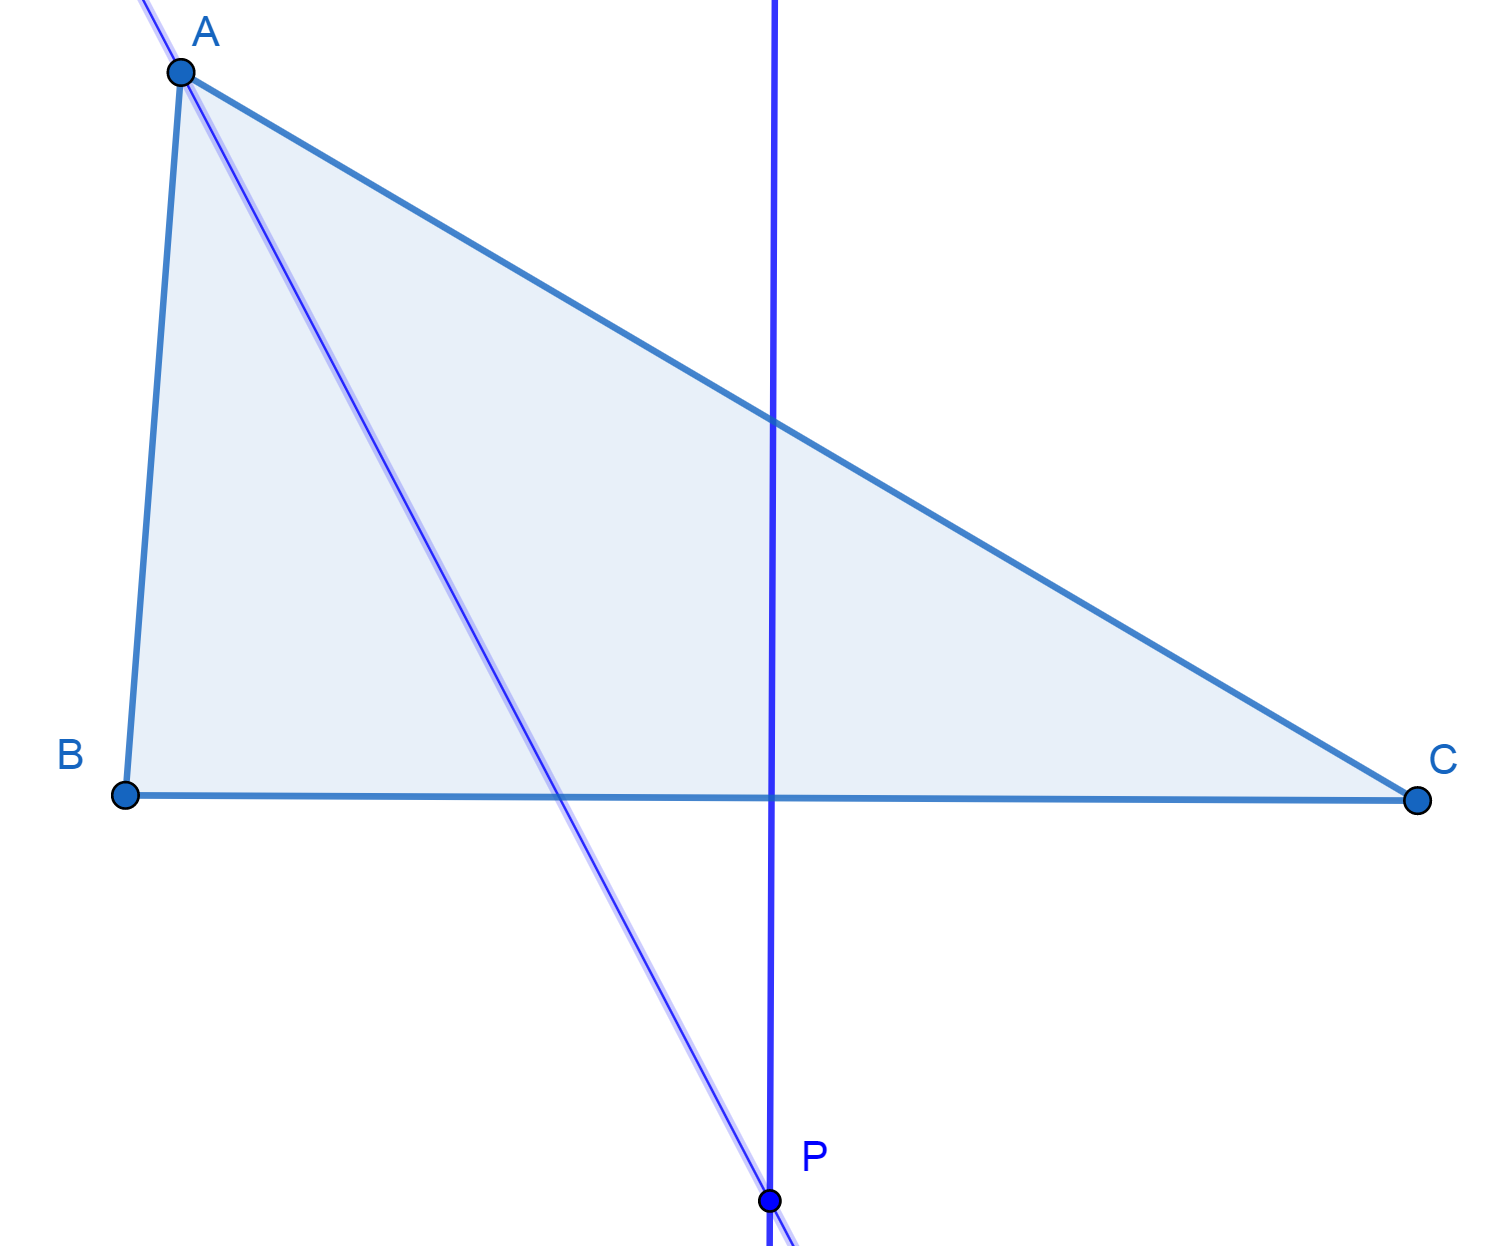
\includegraphics[width=.5\textwidth]{isoceles}
\end{center}

\selectlanguage{english}

%%%%%%%%%%%%%%%%%%%%%%%%%%%%%%%%%%%%%%%%%%%%%%%%%%%%%%%%%%%%%%%
